% This work is licensed under the Creative Commons Attribution-NonCommercial 4.0 International License.
% To view a copy of this license, visit http://creativecommons.org/licenses/by-nc/4.0/
% or send a letter to Creative Commons, PO Box 1866, Mountain View, CA 94042, USA.

% !TEX TS-program = xelatex

\documentclass[../Main/chem532-notes.tex]{subfiles}
\begin{document}

\setcounter{chapter}{5}

\chapter{Basis Sets and Other Practical Aspects of Self-Consistent-Field Calculations}

When we discussed the Roothan equations, we expressed the spatial molecular orbitals $\phi_i(\mathbf{r})$ as a linear combination of basis functions $\{ \chi_\mu(\mathbf{r}) \}$ as
\begin{equation}
\phi_i(\mathbf{r}) = \sum_{\mu} \chi_\mu(\mathbf{r}) C_{\mu i}.
\end{equation}
In this section we will take a look at the mathematical functions that are commonly used to define a basis sets.
Such basis functions have to satisfy a few requirements.
First, they should provide a good approximation to the exact solution of our problem. For example, if we want to study the \ce{H2} molecule, we could use as a basis the atomic orbitals of hydrogen. A finite basis of H atomic orbitals will not give the exact answer for \ce{H2}, but will be close enough to the exact solution.
A second requirement for a good computational basis set is that all integrals required (overlap, kinetic energy, etc.) can be computed analytically. It is possible to use numerical integration to evaluate integrals, but since in practical computations one must calculate around $10^6$ or more integrals, fast analytical integrals are generally preferable.
The last criterion is that the basis set should be systematically improvable. That is, by adding more basis functions we should be able to saturate the basis and represent any well-behaved function with it.

%\section{Slater Basis Sets}
%Slater type orbitals (STOs) generalize the analytic solutions for the hydrogen atom and have the form
%\begin{equation}
%\chi(\zeta, n, l, m) = r^{n - 1} e^{-\zeta r} Y_l^m(\theta, \phi),
%\end{equation}
%where $\zeta$ is the exponent 





\section{Gaussian Basis Sets}
The most important set of basis functions used in quantum chemistry computations are Gaussians. The general form for a \textit{Cartesian} Gaussian function centered at $\mathbf{R} = (X,Y,Z)$ as a function of the electron coordinate $\mathbf{r} = (x,y,z)$ is
\begin{equation}
g(\alpha, \mathbf{r}, l, m, n) = x^l y^m z^n e^{-\alpha (\mathbf{r}- \mathbf{R})^2},
\end{equation}
where $\alpha$ is the exponent of the Gaussian, $(l,m,n)$ are nonnegative integers that determine the shape of the Gaussian function, and $(\mathbf{r}- \mathbf{R})^2$ is the square of the distance from the center.

In the following we will assume for convenience that $\mathbf{R} = 0$, so that we can express the Gaussian in terms of the distance of the electron from the origin, $r = |\mathbf{r}| = \sqrt{x^2 + y^2 + z^2}$.
A Gaussian with spherical symmetry is obtained by setting $l=m=n=0$
\begin{equation}
g(\alpha, \mathbf{r},0,0,0) = e^{-\alpha r^2}.
\end{equation}
Functions that are shaped like p orbitals satisfy the condition $l + m + n = 1$. For example,
\begin{align}
g(\alpha, \mathbf{r},1,0,0) & = x e^{-\alpha r^2},\\
g(\alpha, \mathbf{r},0,1,0) & = y e^{-\alpha r^2},\\
g(\alpha, \mathbf{r},0,0,1) & = z e^{-\alpha r^2},
\end{align}
are p$_x$-, p$_y$-, and p$_z$-like orbitals, respectively.

Notice, however, that when we consider the case $l + m + n = 2$ we can write down \textbf{six} \begin{align}
g(\alpha, \mathbf{r},2,0,0) & = x^2 e^{-\alpha r^2},\\
g(\alpha, \mathbf{r},1,1,0) & = xy e^{-\alpha r^2},\\
g(\alpha, \mathbf{r},1,0,1) & = xz e^{-\alpha r^2},\\
g(\alpha, \mathbf{r},0,2,0) & = y^2 e^{-\alpha r^2},\\
g(\alpha, \mathbf{r},0,1,1) & = yz e^{-\alpha r^2},\\
g(\alpha, \mathbf{r},0,0,2) & = z^2 e^{-\alpha r^2}.
\end{align}
Some of these you will recognize as d functions, for example $g(\alpha, \mathbf{r},1,1,0)$, which is a d$_{xy}$-like function.
Other orbitals like, for example, the d$_{x^2 - y^2}$ can be obtained by taking an appropriate combination of Cartesian Gaussians
\begin{equation}
g(\alpha, \mathbf{r},2,0,0)- g(\alpha, \mathbf{r},0,2,0) = (x^2 - y^2) e^{-\alpha r^2}.
\end{equation}
Interestingly, after we form the five canonical d orbitals out of the six Cartesian Gaussians, we are left with the following linear combination orthogonal to all other five d functions
\begin{equation}
g(\alpha, \mathbf{r},2,0,0)+g(\alpha, \mathbf{r},0,2,0)+g(\alpha, \mathbf{r},0,0,2) = (x^2 + y^2 + z^2) e^{-\alpha r^2} = r^2 e^{-\alpha r^2}.
\end{equation}
This function has spherical symmetry and so it is classified as an s orbital.

Individual Gaussian functions cannot reproduce the shape of atomic orbitals because both near the nucleus, when $\mathbf{r} \approx (0,0,0)$, and far from it, when $|\mathbf{r}| \rightarrow \infty$, they have an incorrect mathematical form due to the Gaussian factor $\exp(-\alpha r^2)$.
To see this point let us compare the s-like Gaussian $g(\alpha, \mathbf{r},0,0,0) = e^{-\alpha r^2}$ with the hydrogen atom s orbital
\begin{equation}
\phi_{1\mathrm{s}}(\mathbf{r}) = N_{1\mathrm{s}} e^{- r},
\end{equation}
where $N_{1\mathrm{s}} $ is a normalization function.
Near the nucleus, $\phi_{1\mathrm{s}}(\mathbf{r})$ has a cusp, while $g(\alpha, \mathbf{r},0,0,0)$ is rounded.
Far from the nucleus instead, Gaussians decay too quickly due to the factor $r^2$ in the exponent. These deficiencies are illustrated in Fig.~\ref{fig:sto_vs_gto}.
\begin{figure}[htbp]
   \centering
   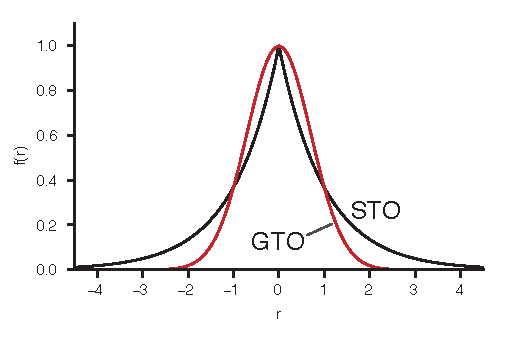
\includegraphics{sto_vs_gto.pdf} % requires the graphicx package
   \caption{Comparison of the hydrogen atom orbital and a Gaussian function.}
   \label{fig:sto_vs_gto}
\end{figure}

To better represent an atomic orbital with Gaussians, it is possible to take a linear combination of Gaussians, also called a contracted Gaussian function.
A general contracted Gaussian $\chi_\mu(\mathbf{r})$ is specified by a set of exponents $\{\alpha_p \}$ and contraction coefficients $\{d_{p\mu}\}$
\begin{equation}
\chi_\mu(\mathbf{r}) = \sum_p g(\alpha_p, \mathbf{r}, l, m, n) d_{p\mu}.
\end{equation}
\begin{figure}[htbp]
   \centering
   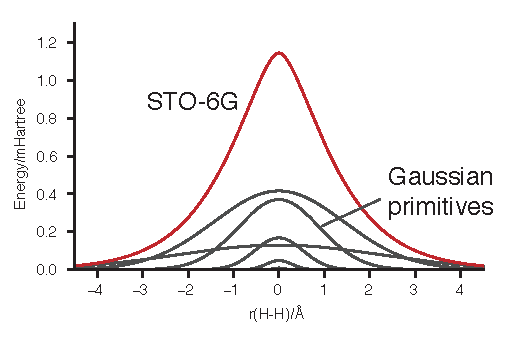
\includegraphics{sto6g.pdf} % requires the graphicx package
   \caption{A Slater type orbital obtained by combining six Gaussian primitive functions (STO-6G).}
   \label{fig:sto6g}
\end{figure}
The Gaussian functions used to construct $\chi_\mu$ are often called \textbf{primitives}.
As an example, consider the following specification for the STO-6G basis set for hydrogen, a contracted basis set obtained by combining 6 primitive Gaussians taken from the EMSL Basis Set Exchange
\begin{verbatim}
!  STO-6G  EMSL  Basis Set Exchange Library   3/19/19 6:19 AM
! Elements                             References
! --------                             ----------
! H - Ne:  W.J. Hehre, R.F. Stewart and J.A. Pople, J. Chem. Phys. 51, 2657
! (1969).

****
H     0 
S   6   1.00
     35.52322122             0.00916359628    ! <-- exponent, coefficient
      6.513143725            0.04936149294    
      1.822142904            0.16853830490    
      0.625955266            0.37056279970    
      0.243076747            0.41649152980    
      0.100112428            0.13033408410    
****
\end{verbatim}
This basis contains Gaussian with exponents that range from 35.5 to 0.1, which when combined together give the function shown in Fig.~\ref{fig:sto6g}.
This function still does not have a cusp, but its form is closer to that of a atomic 1s orbital.

%\section{Convergence of the energy and basis set extrapolation}


\end{document}